\documentclass{article}

\usepackage[dvipsnames]{xcolor}
\usepackage{tikz}
\usetikzlibrary{shapes,arrows}
\usepackage{caption} 
\usepackage[letterpaper]{geometry}
\usepackage{pdfpages}
\usepackage[normalem]{ulem}
\usepackage{wrapfig}
\usepackage{hyperref}

\newcommand{\twsse}{\emph{Time Wizards: The Sober and Serious Edition}}
\newcommand{\tw}{\emph{Time Wizards}}
\newcommand{\sse}{\emph{Sober and Serious Edition}}
\newcommand{\rfe}{\emph{Revised First Edition}}
\newcommand{\vers}{Version $0.1.0 \alpha$}

\tikzstyle{decision} = [diamond, draw, 
    text width=4.5em, text badly centered, node distance=3cm, inner sep=0pt]
\tikzstyle{block} = [rectangle, draw, 
    text width=5em, text centered, rounded corners, minimum height=4em]
\tikzstyle{line} = [draw, -latex']

\definecolor{anongreen}{HTML}{117743}
\newcommand{\anon}[1][]{{\color{anongreen} \textbf{Anonymous}#1}}
\newcommand{\namefag}[2][]{{\color{anongreen} \textbf{#2}#1}}

\AtBeginDocument{\let\textlabel\label}

\begin{document}

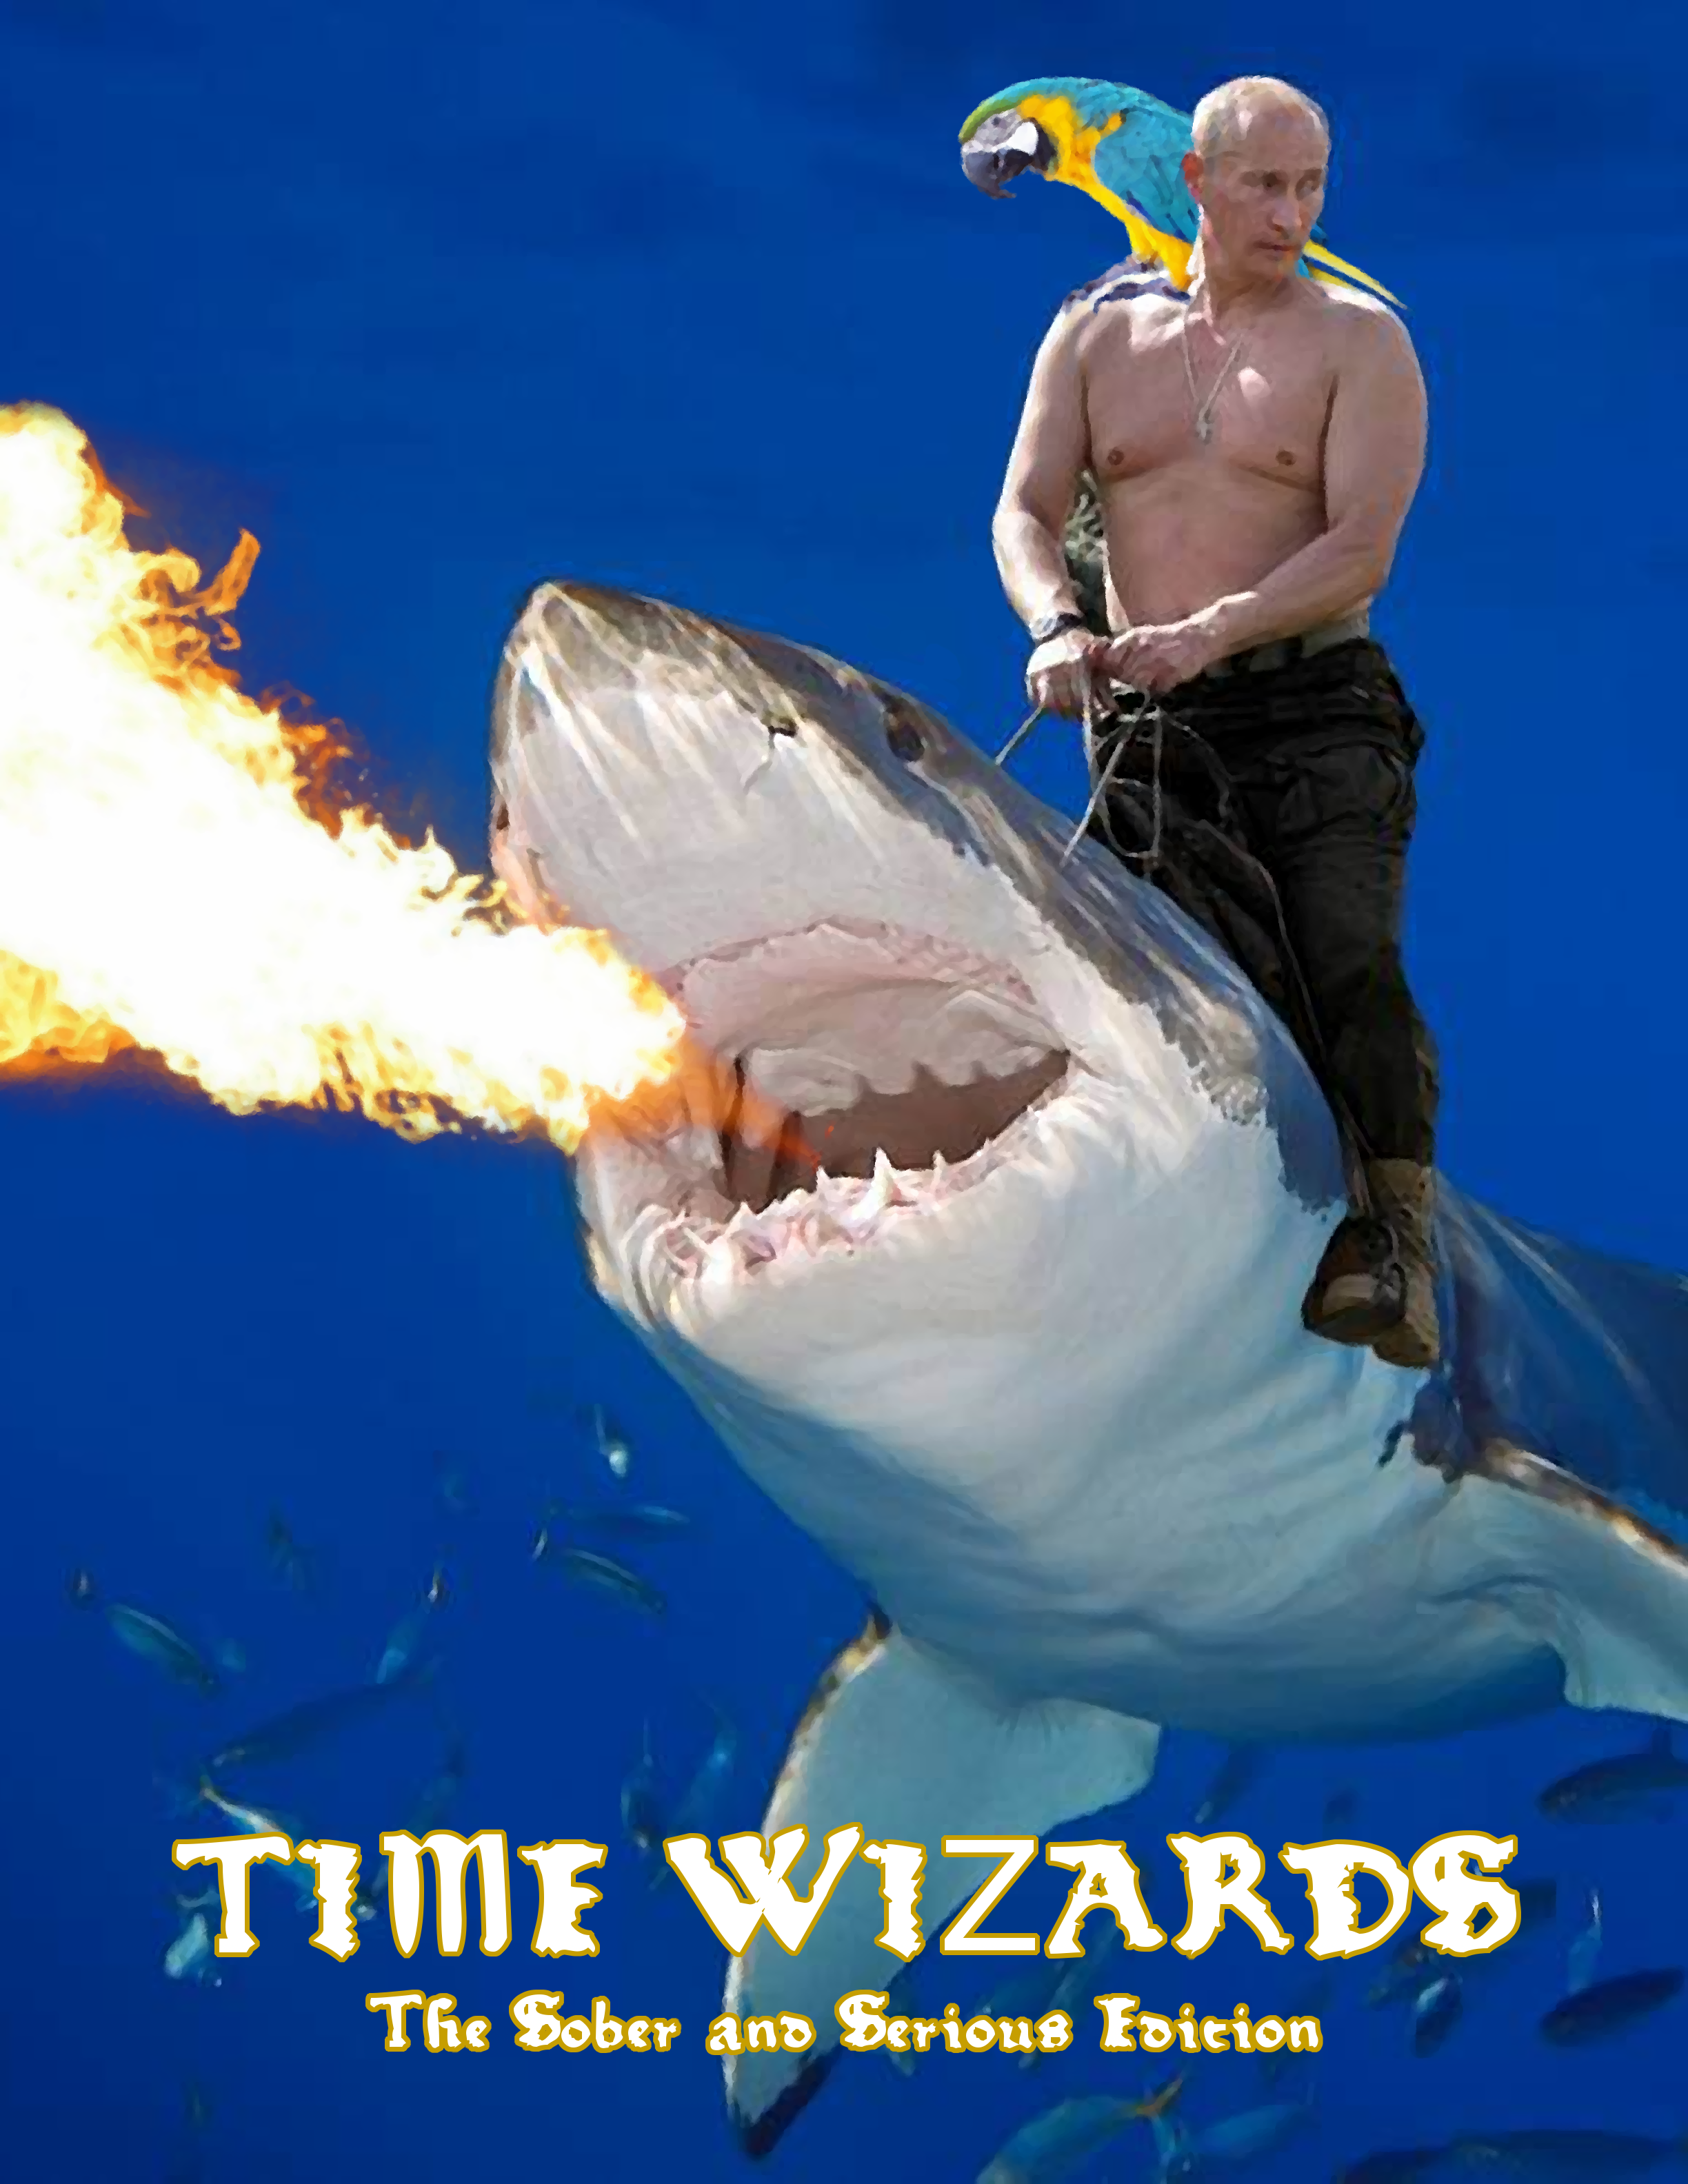
\includepdf[fitpaper]{cover}
\cleardoublepage

\section{Introduction}
Hello, and welcome to \sout{a wall of fucking text} \twsse{}, a game for serious individuals
with serious lives. At least, by the standards of \tw{} players, which is sort of like saying
``a particularly Chaotic sort of paladin'' or ``a very healthy lich''. As the name might 
somewhat jokingly) suggest, \sse{} is an attempt at producing a game with similar potential for
shenanigans as traditional \tw{} while being more accessible to a general tabletop audience.

This ``edition'' is very much a work in progress, and any playtest information you have is very
welcome; \namefag{Time Wizard Archibald}, the main author of this document, can be contacted with
any feedback at \verb|archie.m.vist@gmail.com|. Expect this document to expand and contract as
the rules finalise. Also expect the formatting to improve as I take more time to actually block
things out and organise things.

For reference, this is version \vers{} of \twsse. See versions on the github for version
differences.

\section{Differences from \emph{Time Wizards: Revised First Edition}}
This section assumes some familiarity with \emph{Time Wizards: Revised First Edition}. If you're
playing \tw{} for the first time using \sse{} for some reason, feel free to skip to the next
section.

The basics of character creation remain the same as in \rfe{}: each character selects five ``verb
the noun'' phrases from lists provided by the Time Master, which serve as their Time Wizard
powers. Added in \sse{} are two numeric values, which are given values from 1-9 and must sum to
10. These characteristics determine the scale and variety of effects that a Time Wizard's powers
can achieve. For the particulars on characteristics and their uses, see the \textbf{Choose
Characteristics} section under \textbf{Character Creation}.

In terms of mechanics, the classic \rfe{} of \tw{} is a completely different game from \sse{}.
In particular, the entire dice slap system from classic \tw{} has been removed; while some may
say this removes a characteristic part of what makes a game of \tw{} what it is, it was removed
for several reasons: first and foremost, to make the game more accessible. As a rule, people
(even many fa/tg/uys) tend to avoid physical pain; as such, most any other RPG system would be
easier to pitch to a group than a game of \rfe{} or other slap system \tw{}.

Further, a slap system offers a significant advantage to those with stronger physical
characteristics, such as longer arms or better pain tolerance. As \namefag{Time Wizard Archibald}
has the physical constitution of a gnome who bathes in burnt othur fumes, and many other people
do not, switching to a strictly dice-based system evens the playing field for him and others with
delicate lady hands.

For the new power mechanics, see the \textbf{Time Moments} section.

The referenced sections should be sufficient for someone familiar with \emph{Time Wizards:
Revised First Edition} to play \sse{}.

\section{Setting Up}
First, it is absolutely pivotal to begin a game of \tw{}, no matter what edition, with a loud
and joyous cry of \emph{``¡mientras tanto, los MAGOS DEL TIEMPO!''}. If you can't even pretend
to speak Spanish, any local equivalent of ``Meanwhile, the Time Wizards!'' is acceptable.

Conventional \tw{} also suggests the addition of one silly house rule, referred to as a Doctrine,
by each player. \twsse{} does not officially require Doctrines, but their addition can bring
excellent further antics with an experienced groups. Doctrines can be strictly mechanical
(``reroll all threes''), strictly social (``every time you say sentence with three or more Qs
in it, take a drink''), or a hybrid of the two (``every time a player swears, 1d6 sheep appear
surrounding their character'').

\subsection{Character Creation} \label{ssec:creation}
Each player in a game of \tw{} controls a single Time Wizard: mighty masters of time and space
who warp reality to their will in both highly-specific yet completely open-ended ways. Prior to
their sudden, unexpected ascendancy to Time Wizardhood, a Time Wizard is an individual going
about an ordinary day who is suddenly and instantaneously imbued with mighty eldritch powers,
based on some of the last things they did as a mortal man.

Note that they must be going about an ordinary day, no matter how extraordinary the character
may be: they could be the ruler of all known space, but the day they awakened to Time Wizard
powers would be the day they went to a wine tasting and caught up on paperwork. It is for this
reason that Theodore Roosevelt cannot become a Time Wizard. Theodore Roosevelt does not need to
become a Time Wizard.

\subsubsection{Determine Powers} \label{ssec:get-powers}
First, when creating your Time Wizard, determine what your character's mortal life was like;
this lets you give the TM ideas about what your character was doing. The TM then proceeds to
describe the events of your character's life through sets of phrases in the general form
``verb the noun'': that is, performing some action on some object. The size and number of the
sets is up to the TM's discretion, but each should contain at least five phrases. If a player
rejects a set, the TM must provide another; players can choose their powers from exactly one
set, and can only choose one of the two most recent sets provided by the TM. Reject your first
two sets, for instance, and you cannot go back and choose the first after you hear the third.

\subsubsection{Determine Characteristics} \label{ssec:get-characteristics}
With your character's five powers chosen, you must then allocate your Time Wizard's
characteristics. Time Wizards are rather simple entities, with two characteristics: Will,
representing the Time Wizard's mental fortitude, and a second stat which represents their
ability to understand and use their Time Wizard powers. The name of this stat is chosen by each
Time Wizard based on something in their past life; for instance, a stage magician may attribute
their newfound powers to their Showmanship, while a bodybuilder might attribute it to their
Musculature. For consistency, we will call this a Core Attribute; it can be any attribute of the
character, usually something they see as a definitive aspect of themselves. A Time Wizard's two
characteristics must sum to 10: if Captain Ahab the Time Wizard has 7 Desire To Slay The Whale,
he must then have 3 Will.

Time Wizards have access to two pools of power: their Power pool, which is determined by Will,
and their Posits, which are determined by their Core Attribute. A time wizard has a maximum of
five times their Will in Power, and has three times their Core Attribute plus two in Posits.
A ``balanced'' Time Wizard has 5 Will and 5 Core Attribute, for a total of 25 Power and 17
Posits. A full listing of Time Wizard attribute choices and their results is given in
Table~\ref{tab:cawill}: CA and Will Values.

To ``Posit'' means to put forward a logical proposition, and is also a homophone for ``pause
it'' if you have the right accent. This suggests the function of a Posit: to declare a Time
Moment and to expand the function of your Time Wizard powers beyond their mundane trappings.
Declaring a Time Moment, dilating time, and making outlandish prepositions for your Time Wizard
powers all require at least one Posit be spent.

\begin{wraptable}{r}{0.5\textwidth}
   \caption{CA and Will Values}
   \label{tab:cawill}

   \begin{tabular}{cc|ccc}
   \textbf{CA} & \textbf{Will} & Posits & Power & Dice Cap\\ \hline
      1 & 9 &  5 & 45 &  3\\
      2 & 8 &  8 & 40 &  4\\
      3 & 7 & 11 & 35 &  5\\
      4 & 6 & 14 & 30 &  6\\
      5 & 5 & 17 & 25 &  7\\
      6 & 4 & 20 & 20 &  8\\
      7 & 3 & 23 & 15 &  9\\
      8 & 2 & 26 & 10 & 10\\
      9 & 1 & 29 &  5 & 11
   \end{tabular}
\end{wraptable}

Power is more straightforward: you can spend a point of power to either add a single d6 to your
roll to activate a power. By default, you roll 2d6; the maximum number of dice you can add is
equal to your Core Attribute. The maximum number of dice you can roll is given in the nearby
table under Dice Cap.

In general, have more Will if you think you want broad, reliable powers that are relatively
straightforward, and have more Core Attribute if you want powers to be highly versatile at the
cost of reliability.

With your characteristics and powers determined, your Time Wizard is ready to play!

\subsection{The Scenario} \label{ssec:scenario}
When every party member has finished character creation, the Time Master outlines the situation
and objective of the party. \twsse{}, like all forms of \tw{}, is not designed for long
campaigns\footnote{But if you run one, storytime that shit.}; generally, you'll be playing for
an hour or so after another game, or to kill time during the day. It's highly recommended to
have a straightforward objective for the players to focus their energies on, or else the game
drags for lack of purpose.

A good scenario can be anything from ``Liberate the world's supply of croissants'' to ``Kill
Hitler'' to ``Steal the Hope Diamond (to pay your rent)''. (These are all from actual games of
\tw{} I have played or TM'd: the first and third in \rfe{}, the second being the inaugural game
of \sse{}.) Any task that isn't trivially simple can be complicated by the sheer chaos that a
group of Time Wizards will inevitably bring to any goal; the fun of \tw{} isn't achieving the
objective, it's everything that happens along the way.

\section{Time Moments} \label{sec:time-moment}
With player characters and a scenario, it's time to play the game. The Time Wizards can bumble
around in an active universe and try and do things like ordinary people; there aren't really
rules for this right now, so it's largely to the TM's discretion how events occur in normal time
(if they really matter at all). Essentially, normal-time gameplay is made up of two things:
waiting for a Time Moment, and the immediate aftermath of a Time Moment.

A Time Moment is a frozen instant in time, during which the Time Wizards may use their powers.
Movement and direct action are impossible; the only thing that can happen during a Time Moment
is the use of Time Wizard powers. \hyperref[fig:timemoment]{Figure \ref*{fig:timemoment}: Flow
of a Time Moment} shows the general structure of a Time Moment in \twsse{}.

\begin{figure}
   \caption{Flow of a Time Moment}
   \label{fig:timemoment}

   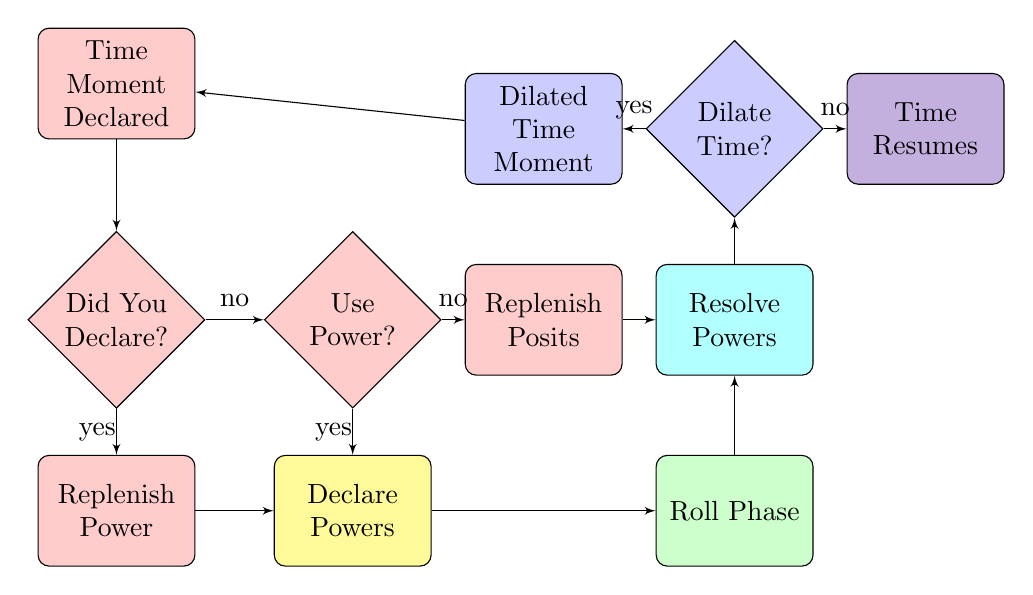
\begin{tikzpicture}
      \node [block, fill=red!20] (init) {Time Moment Declared};
      \node [decision, below of=init, fill=red!20] (determine) {Did You Declare?};
      \node [decision, right of=determine, fill=red!20] (decide) {Use Power?};
      \node [block, right of=decide, node distance=0.2\textwidth, fill=red!20] (posits)
         {Replenish Posits};
      \node [block, below of=determine, node distance=0.2\textwidth, fill=red!20] (power)
         {Replenish Power};
      \node [block, below of=decide, node distance=0.2\textwidth, fill=yellow!40] (declare)
         {Declare Powers};
      \node [block, right of=declare, node distance=0.4\textwidth, fill=green!20] (roll)
         {Roll Phase};
      \node [block, above of=roll, node distance=0.2\textwidth, fill=Cyan!30] (resolve)
         {Resolve Powers};
      \node [decision, above of=resolve, node distance=0.2\textwidth, fill=blue!20]
         (dilate) {Dilate Time?};
      \node [block, right of=dilate, node distance=0.2\textwidth, fill=RoyalPurple!30] (done)
         {Time Resumes};
      \node [block, left of=dilate, node distance=0.2\textwidth, fill=blue!20] (new)
         {Dilated Time Moment};

      \path [line] (init) -> (determine);
      \path [line] (determine) ->
         node [left of=start, node distance=0.02\textwidth] {yes} (power);
      \path [line] (determine) ->
         node [above of=start, node distance=0.02\textwidth] {no} (decide);
      \path [line] (decide) ->
         node [left of=start, node distance=0.02\textwidth] {yes} (declare);
      \path [line] (decide) -> node [above of=start, node distance=0.02\textwidth] {no} (posits);
      \path [line] (power) -> (declare);
      \path [line] (posits) -> (resolve);
      \path [line] (declare) -> (roll);
      \path [line] (roll) -> (resolve);
      \path [line] (resolve) -> (dilate);
      \path [line] (dilate) -> node [above of=start, node distance=0.02\textwidth] {yes} (new);
      \path [line] (dilate) -> node [above of=start, node distance=0.02\textwidth] {no} (done);
      \path [line] (new) -> (init);
   \end{tikzpicture}
\end{figure}

The colours in the figure indicate a grouping according to the section in the rules: red is
covered under \hyperref[ssec:begin-moment]{Beginning a Time Moment}, yellow under \hyperref
[ssec:power-declaration]{Power Declaration}, green under \hyperref[ssec:roll-phase]
{The Roll Phase}, cyan under \hyperref[ssec:resolve-power]{Power Resolution}, blue under 
\hyperref[ssec:time-dilation]{Time Dilation}, and purple under \hyperref[ssec:end-moment]{Ending
a Time Moment}.

\subsection{Beginning a Time Moment} \label{ssec:begin-moment}
A Time Wizard may declare a Time Moment at any time for the cost of one Posit; if they have no
Posits available, they cannot declare a Time Moment, and are helpless save for the intervention
of their fellow Time Wizards. As soon as the Time Moment is declared, time freezes and the
Time Wizards step away from reality, ready to work their havoc upon it.

The Time Wizard who declares the Time Moment regains one third of their maximum Power, rounded
down, upon declaration; however, they must declare a power to use during this Time Moment. Other
Time Wizards can either choose to declare a power or to regain one Posit for each power used in
this Time Moment.

\subsection{Power Declaration} \label{ssec:power-declaration}
The Time Wizards who decide to participate in a Time Moment must then declare which of their
five powers they intend to use, and the amount of their Power they intend to use. One point of
Power adds one die to the amount rolled, or increases the size of the effect. Effect sizes are
given in \hyperref[tab:powersize]{Table \ref*{tab:powersize}: Power to Size Guidelines}; it'
good to ask the TM for specific sizes of objects to determine the Power that needs to be spent
to influence it.

\begin{wraptable}{r}{0.5\textwidth}
   \caption{Power to Size Guidelines}
   \label{tab:powersize}

   \begin{tabular}{c|c}
      \textbf{Power Spent} & {Size Limit}\\ \hline
      0 & The power's user only\\
      1 & A person\\
      2 & A house or building\\
      3 & A city block\\
      4 & A small town\\
      5 & A large city\\
      6 & A small country\\
      7 & A continent\\
      8 & A planet\\
      9 & A star system\\
      10 & A galaxy\\
      11 & The entire universe
   \end{tabular}
\end{wraptable}

Further Power-to-area tiers can be added at the TM's discretion. So long as the Time Wizard has
the power in their pool, there is no limiting factor for spending it on area of
effect.\footnote{Yes, we know it's actually a volume of effect.} Suggested values for 12 Power
include the entire multiverse, if such a thing is pertinent to your game, or a cluster of
related universes if the multiverse is truly large. Another use for high Power would be to
interfere with other games of \tw{} occurring in the same area, so long as your Time Masters
have an understanding.

When using Power to increase the number of dice rolled beyond the initial 2d6, note that the
number of added dice cannot exceed the Time Wizard's Core Attribute score. The maximum number
of dice a Time Wizard with a given attribute spread can roll is given in Section 3, in
\hyperref[tab:cawill]{Table \ref*{tab:cawill}: CA and Will Values}.

\subsection{The Roll Phase} \label{ssec:roll-phase}
Once the amount of Power used by each Time Wizard is determined, each Time Wizard rolls their
chosen number of dice, beginning with the player who declared the Time Moment and moving through
the rest of the active Time Wizards in some order from there. (While the TM can decide this, we
suggest clockwise order or some other standard to keep things somewhat consistent.) These rolls
are opposed by another roll from the TM, based on the Order of the situation.

The more ordered and controlled a situation is, the more the Time Wizards thrive in it. If a
situation is already frantic and chaotic, the relative influence of the Time Wizards'
reality-breaking powers isn't as obvious, and the universe puts up less resistance. The amount
of resistance to Time Wizard interference exhibited by the environment is referred to as the
Order Rating, or simply Order; this is set by the TM, and changes based on the actions of the
players. Maintaining a low Order Rating allows Time Wizards to achieve more success for less
Power, but also places them at risk when time is in motion.

Normally, assuming there's no Wrath involved, the TM rolls 1d6 for each point of Order. The
winner of the roll is whichever player has a higher number; in the event of a tie, the winner
goes to whichever player rolled fewer dice. In the event that both of these are a tie, the
Time Wizard succeeds. When a Time Wizard succeeds, they get to choose how their power resolves
and they gain a point of Wrath; when a Time Wizard fails, the TM chooses how the power resolves.

\subsubsection{Wrath} \label{sssec:wrath}
Wrath is the representation of how much reality is sick of a given Time Wizard's shit. For
every successful roll against the TM, a Time Wizard gains a point of Wrath. When a Time Wizard
attempts to activate a power, the TM may use accumulated Wrath one of two ways: a single point
of Wrath will add one die to the roll against that power, or will increase the size of all dice
rolled against that power: a single point of Wrath will have the TM roll d8s, two will see
d10s, three will see d12s, and four will see d20s. This allows the TM to hijack particularly
useful Time Wizard powers and gain revenge on highly successful players even at low Order.

If Captain Ahab the Time Wizard were to ``hoist the rigging'' with an Order Rating of 2 and he
had accumulated five points of Wrath, the TM could spend three points to roll 4d8 instead of
2d6, greatly improving his odds of winning the roll. These three points are consumed regardless
of the outcome, leaving Captain Ahab with two points of Wrath (if he loses) or three points of
Wrath (the two remaining, plus the one gained by a successful roll).

\subsection{Resolving Powers} \label{ssec:resolve-power}
Depending on the outcome of rolling for power activation, either the Time Wizard or the TM
decides how a given power resolves. Every power, you recall, is of the form ``verb the noun'':
to resolve a power, the player or TM must describe how some intended result is an action
matching the verb and noun from the power: for instance, ``unwrap the cheeseburger'' could be
used to shred the unnecessary bits of a loaf of bread and a cow, leaving only a cheeseburger
behind, or could be used to tear apart the cosmic essence of a cheeseburger to turn it into
an eldritch hand grenade. Time Wizard powers are very versatile, if you have the right argument.

In general, it costs a Time Wizard one Posit to declare that one object or one action is some
different action. For instance, it does not cost a Posit to declare that a crate is a box, but
declaring that a rocket launcher (which has a scope on it) is itself a scope would cost one
Posit. At the group's discretion, Posits can also be charged for highly general powers, such as
``ready the materials'' or ``make the delivery'', in order to maintain some illusion of balance.
The total number of Posits which can be spent on a single resolution is the Time Wizard's Core
Attribute value.

When the TM resolves a power, they are not limited by Posits and Core Attribute, but must keep
the effect pertinent to the ability at hand and within the same range specified when the Time
Wizard first declared their power.

Resolve powers in the order that dice were rolled. When all powers have been resolved, the
players have a choice: either have the Time Moment end, causing all consequences from it to
occur, or to enter Time Dilation.

\subsection{Time Dilation} \label{ssec:time-dilation}
At the end of a Time Moment, if circumstances are unfavourable to the Time Wizards, one may
choose to spend additional Posits to produce a Time Moment inside a Time Moment. A Dilated Time
Moment behaves in most respects similarly to a Time Moment, with some slight differences.

First, each layer of Time Dilation increases the number of Posits needed to declare the dilation
by 1. This means that the first layer of Time Dilation requires two Posits; if circumstances are
still unfavourable, dilating a second time would require three, and so on. This increased cost
makes it difficult to repeatedly dilate time until a perfectly desirable outcome is obtained.

Dilating Time, unlike declaring a regular Time Moment, does not restore any of the declaring
Time Wizard's Power, nor does it restore any Posits to inactive Time Wizards. Again, the purpose
of this is to prevent infinite time dilation loops, and to make resolving a Time Moment better
to allow resources.

Finally, all effects of powers in dilated time are amplified, increasing for each level of
dilation. For instance, a simple ``water the flowers'' that would, in a standard Time Moment,
produce a warm sunshower instead produces a torrential downpour and flash floods when time is
dilated. If time were dilated again, it might wash away an entire landmass, or flood the entire
world. The exact nature of the effect increase is up to the resolving player and the TM.

\subsection{Ending a Time Moment} \label{ssec:end-moment}
Whether Time Dilation happens or not, the Time Moment must end, and reality then deals with the
consequences of the Time Wizards' actions. Return to the top of the Playing the Game section
until the Time Wizards complete their objective.

\section{Credits}
As a whole, \twsse{} belongs to the people of /tg/. All work is done on the shoulders of giants,
and this document wouldn't be possible without a grand history of shenanigans that I can only
wish I had a part in.

\tw{} would not exist as it does today were it not for \namefag[!ScSfaqO.RY]{DM Kroft} regaling
/tg/ with his tales of shenanigans, and would not exist at all were it not for a bold unknown
individual in Kroft's group who shouted the first ``Mientras tanto, los MAGOS DEL TIEMPO!'' over
pizza. The creators are named in \emph{Classic Edition} as Cristián Andreu (\namefag{DM Kroft}
himself), Gonzalo Jimenez and Alain Raymond, so buy those guys a beer if you see them. They
deserve it.

\emph{Time Wizards: First Edition} was compiled from the imagination of \anon{} by
\namefag{Art\_Wizard}, providing the first publicly-available ruleset for the game.

\emph{Time Wizards: Revised First Edition} was in turn developed from \emph{First Edition} by a
valiant \anon{}, providing the first full version of \tw{} to /tg/ that is in the form of a
structured, presentable rulebook. \rfe{} remains the primary inspiration for \sse{}, as it is the
form of \tw{} with which I was familiar prior to pitching the idea for a reformed version to
\namefag{Social Techpriest} and the other members of our gaming group.

Further mention should be given to \emph{Time Wizards!} or \emph{Time Wizards: Classic Edition},
the original rules as collected and posted by \namefag[!ScSfaqO.RY]{DM Kroft} in a later thread,
and \emph{Time Wizards: Advanced Edition}, which attempted to reconcile the rules of \rfe{} and
\emph{Classic Edition}. I have not played \emph{Classic} or \emph{Advanced}, but they're still
\tw{} games at heart and I'd be curious to see someone who's played multiple versions compare
them.

The rules of \twsse{} are largely the efforts of \namefag{Social Techpriest}. This document was
written and formatted (such as it is) by \namefag{Time Wizard Archibald}, but giving me credit
for any part of \tw{} is sort of like giving credit for the Empire State Building to a guy who
happened to take a photo of it.

Credit for the cover image and title goes to \anon{} of /tg/.

\section{Future Plans}
First and foremost, I need to typeset this document up nicer so it's not a seamless wall of text
and has nice little things like examples and coloured boxes. Everyone likes coloured boxes.

\end{document}